\documentclass[11pt,a4paper]{article}

\usepackage[margin=2.3cm]{geometry}
\usepackage{amsmath,amssymb}
\usepackage{graphicx}
\usepackage{booktabs}
\usepackage{xcolor}
\usepackage{enumitem}
\usepackage[hidelinks]{hyperref}
\usepackage{caption}

\emergencystretch=1.5em
\captionsetup{font=small,labelfont=bf,width=.92\textwidth}
\setlength{\parskip}{4pt plus 1pt}
\setlength{\parindent}{0pt}

\newcommand{\code}[1]{\texttt{#1}}
\newcommand{\dv}[1]{diverged (#1)}
\newcommand{\bst}[1]{\textbf{#1}}

\title{Stabilizing RBLapSum \code{through\_rank\_kappa}\\[2pt]
\large Research note: kernel temperature, learning rate, output
normalization and support-gradient scale}
\author{}
\date{2026-09-21/22.}

\begin{document}
\maketitle
\vspace{-2em}

% ============================================================
\section{Purpose and summary of conclusions}
% ============================================================

RBLapSum with the kappa correction is usable but not unconditionally stable:
at $K=128$ and $T=1$ it destabilizes within a few thousand steps. Four
interventions are available, and they act on different parts of the
mechanism identified earlier
(\code{docs/scale-dynamics-note-neutral.tex}): broadening the kernel
($T=2$) lowers the surrogate gain, lowering the learning rate shrinks both
the signed drift and the second-order heating, an RMSNorm on each
bottleneck's output removes the depth amplification of the score scale, and
scaling the support term down attenuates the boundary-exchange gradient
directly.

This note compares all four against the untouched baseline on the same
six $(K,J)$ configurations, and asks which one stabilizes training and
which one converges best.

Conclusions:

\begin{itemize}[leftmargin=1.4em]
\item \textbf{All four interventions stabilize.} The baseline diverges in
the two $K=128$ configurations, at steps 1680 and 2200. Every other arm
reaches 20k steps in all six configurations; no divergence was observed in
any of the 24 intervention runs. Stabilization alone therefore does not
separate the four -- the cost of stabilizing does.

\item \textbf{The output RMSNorm is the best intervention on both counts.}
It converges best in five of six configurations, including both
configurations the baseline cannot survive, and its $1.4294$ at
$(K,J)=(128,384)$ is the best value in the comparison. It is also the only
arm that stabilizes without a measurable accuracy cost.

\item \textbf{Broadening the kernel is a close second} and needs no
architectural change: within $\pm0.043$ nats of the baseline wherever the
baseline survives, and $0.030$--$0.038$ nats behind the RMSNorm in the
$K=128$ rows it rescues.

\item \textbf{Lowering the learning rate stabilizes by training less.} It
is last in all six configurations, $0.080$--$0.155$ nats behind the
RMSNorm.

\item \textbf{Scaling the support gradient to $0.3$ stabilizes reliably but
costs accuracy.} It never diverges, but it is $0.005$--$0.063$ nats behind
the RMSNorm and is worse than the untouched baseline in every
configuration where the baseline survives.

\item \textbf{The RMSNorm also helps the hard bottleneck}, which has no
surrogate gradient and no instability to fix: $1.6022$ against $1.6162$ at
$K=32$ and $1.4232$ against $1.4298$ at $K=512$. It is therefore not a
surrogate-specific crutch.
\end{itemize}

% ============================================================
\section{Setup}
% ============================================================

Thirty runs, all RBLapSum \code{through\_rank\_kappa} under full
magnitude--direction decoupling, with the architecture, data, optimizer,
schedules and seed of the earlier campaigns (8$\times$768, \code{abs\_topk}
over $N=1536$ features, \code{residual\_out} placement, batch
$96\times512$ tokens, 20k steps, $b_0=0$).

Six configurations,
\[
(K,J)\in\{(32,32),\,(32,480),\,(64,64),\,(64,448),\,(128,128),\,(128,384)\},
\]
each under five arms:

\begin{center}\small
\begin{tabular}{llll}
\toprule
arm & $T$ & lr & change \\
\midrule
baseline           & 1 & $6\times10^{-4}$ & --- \\
$T=2$              & 2 & $6\times10^{-4}$ & wider kernel \\
lr $2\times10^{-4}$ & 1 & $2\times10^{-4}$ & smaller steps \\
post-norm          & 1 & $6\times10^{-4}$ & RMSNorm on each bottleneck's output \\
support grad $0.3$ & 1 & $6\times10^{-4}$ & \code{rblapsum\_support\_scale}$=0.3$ \\
\bottomrule
\end{tabular}
\end{center}

The first four arms ran on one 8-GPU machine (24 runs, names
\code{ca\_rout\_rblapsum\_kappa\_*\_stab\_*}); the support-gradient-scale arm ran on
a second machine (6 runs, \code{ko\_rout\_rblapsum\_kappa\_*\_supp03\_*}),
along with two hard-AbsTopK runs used for the last conclusion above.

Two implementation notes. The output RMSNorm
(\code{activation\_bottleneck.post\_norm}) is applied inside the bottleneck
module, and the bottleneck whose output already feeds a norm --
\code{residual\_out} in the final block, ahead of \code{norm\_f} -- is
exempt. The support-gradient scale multiplies the boundary-exchange term $g_s$
\emph{after} the mode correction, so the zero-sum structure of
\code{through\_rank\_kappa} is preserved and the term is uniformly
rescaled; the hard task path is untouched, so the scale interpolates
between the full surrogate ($1.0$) and the plain hard-TopK backward
($0.0$).

A run is stopped and recorded as diverged when its training CE becomes
non-finite, stays above its own best plus $2.5$ nats for 800 consecutive
steps, or stays above $7.0$ for 300 steps after step 1500. The window is
relative to each run's own best, so the slower low-learning-rate arm is not
penalized for being behind.

% ============================================================
\section{Results}
% ============================================================

\begin{center}\small
\begin{tabular}{lccccc}
\toprule
$(K,J)$ & baseline & $T=2$ & lr $2\times10^{-4}$ & post-norm & support grad $0.3$ \\
\midrule
$(32,32)$   & 1.5521 & 1.5492 & 1.6709 & \bst{1.5310} & 1.5847 \\
$(32,480)$  & \bst{1.4900} & 1.4943 & 1.6168 & 1.5370 & 1.5419 \\
$(64,64)$   & 1.5281 & 1.5142 & 1.6376 & \bst{1.4834} & 1.5348 \\
$(64,448)$  & 1.4661 & 1.4727 & 1.6006 & \bst{1.4538} & 1.5092 \\
$(128,128)$ & \dv{1680} & 1.4802 & 1.5970 & \bst{1.4423} & 1.5037 \\
$(128,384)$ & \dv{2200} & 1.4598 & 1.5843 & \bst{1.4294} & 1.4926 \\
\bottomrule
\end{tabular}
\end{center}

Final validation CE after 20k steps, or the step at which the divergence
guard stopped the run. Best value per configuration in bold.

\begin{figure}[h]\centering
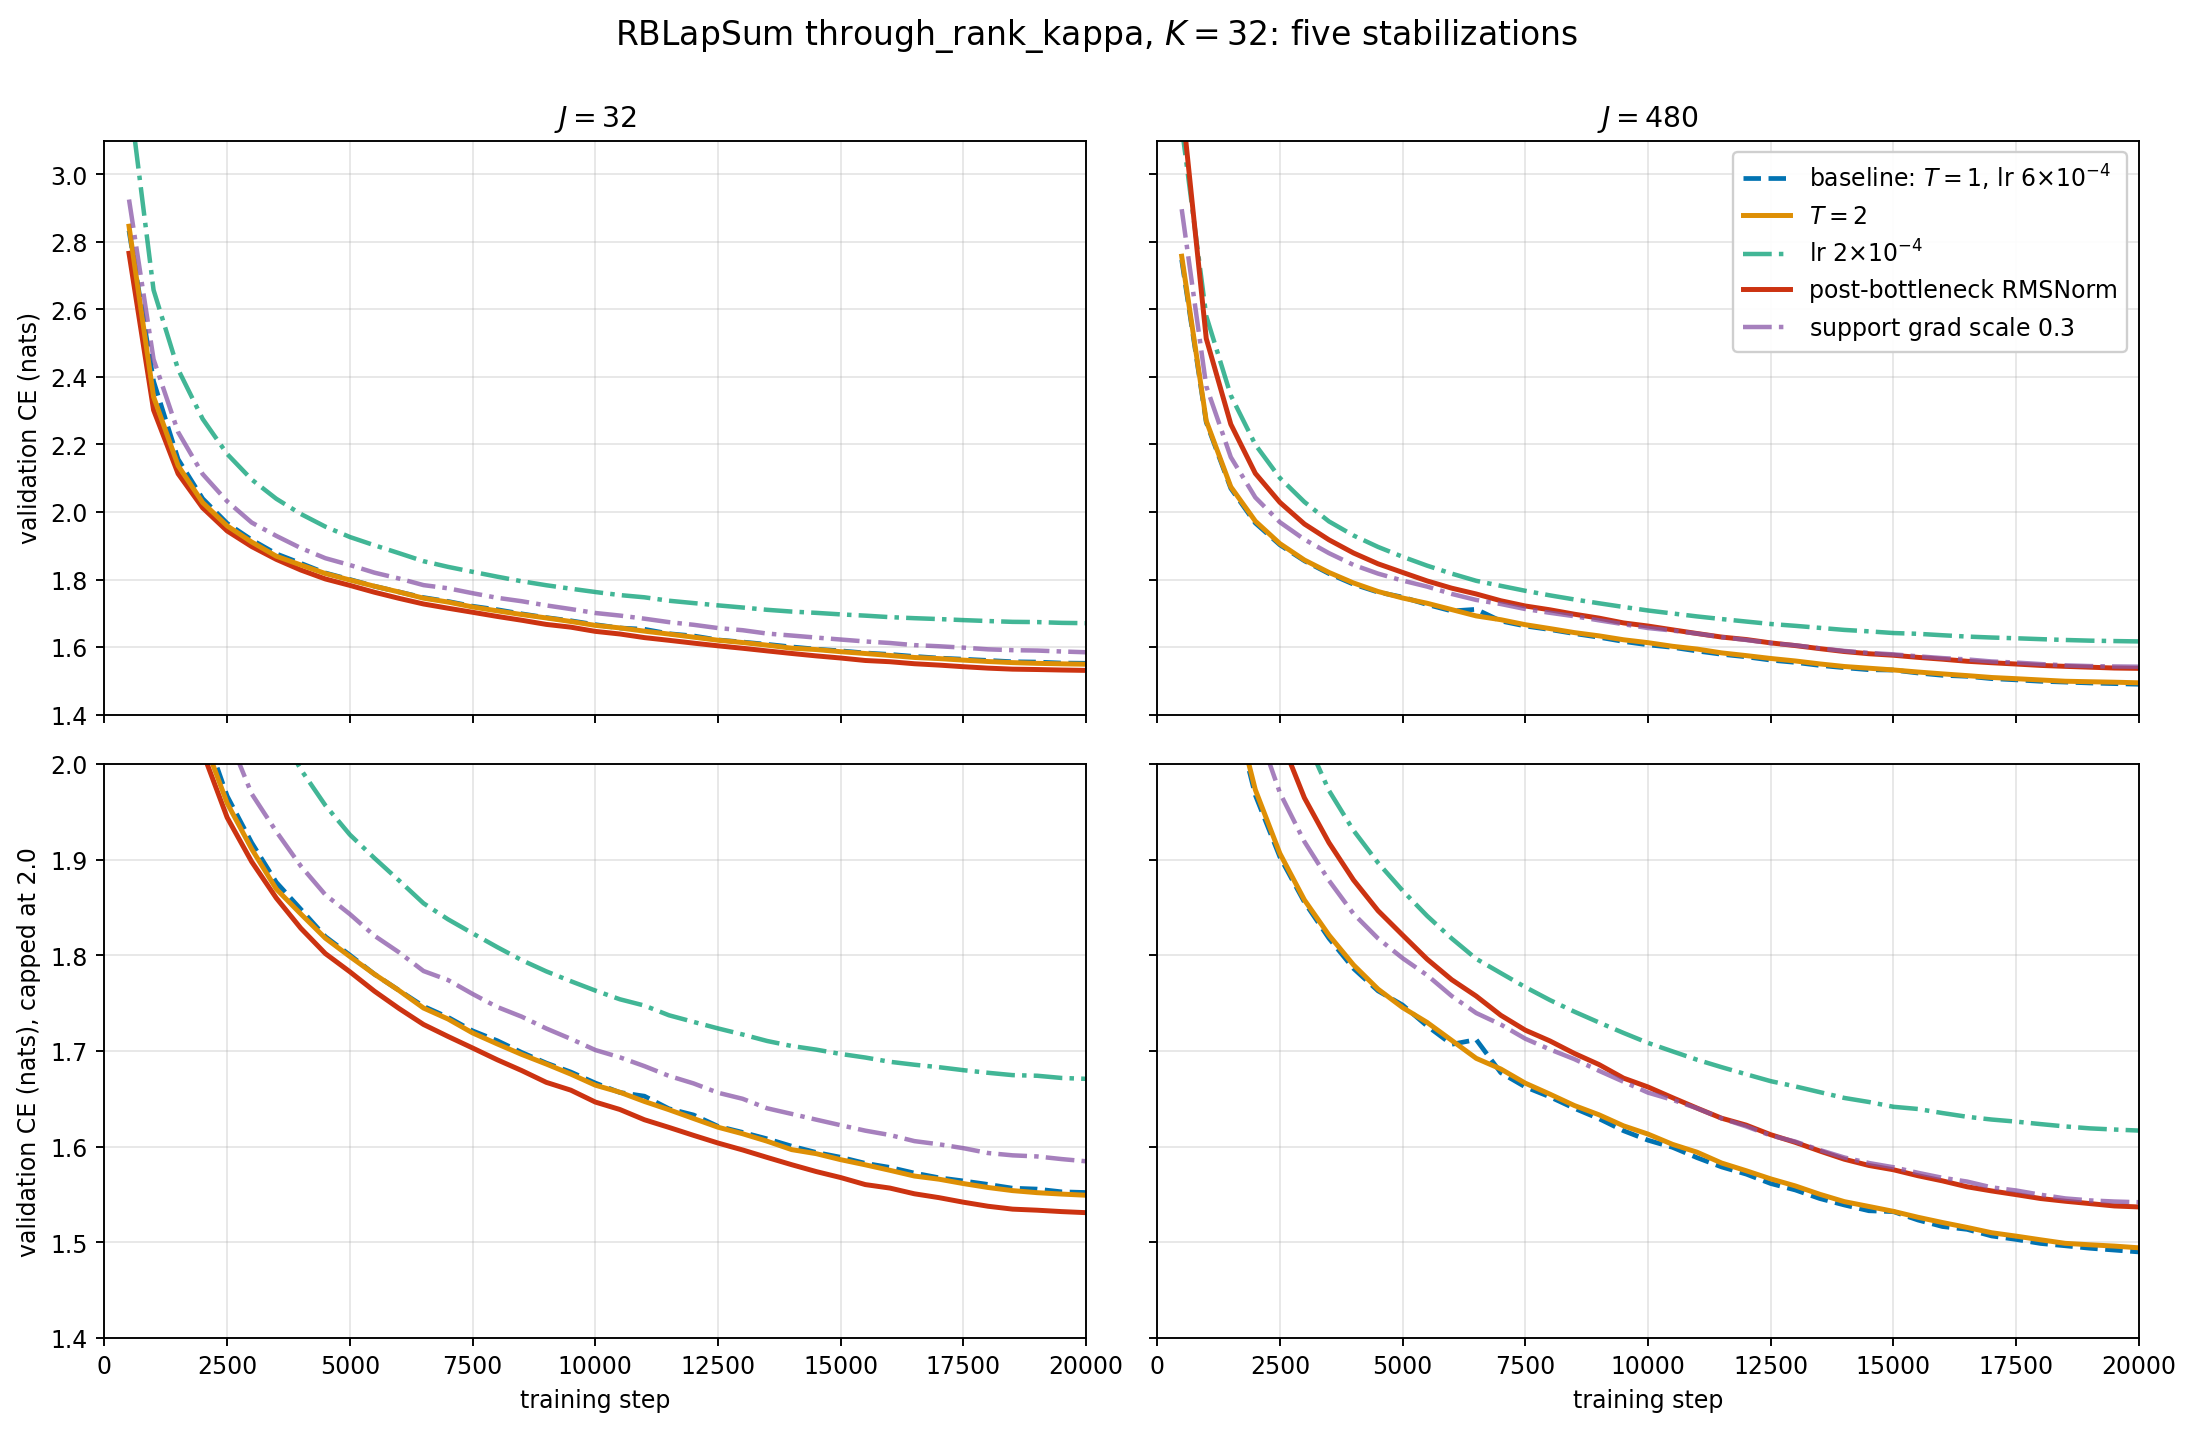
\includegraphics[width=\textwidth]{figures/stab_k32.png}
\caption{$K=32$: smaller candidate window on the left, larger on the
right; the lower row repeats each panel with the vertical axis capped at
2.0 nats. Colour encodes the arm and line style its kind: the untouched
baseline is dashed, the two arms that stabilize without an accuracy cost
($T=2$ and the output RMSNorm) are solid, and the two attenuating arms
(reduced learning rate, support-gradient scale) are dash-dotted and
slightly transparent. Every arm survives here, so this
configuration measures cost rather than stabilization: the baseline and
$T=2$ curves are indistinguishable, the output RMSNorm wins at $J=32$ but
loses $0.047$ nats at $J=480$, and the reduced learning rate is clearly
behind throughout.}
\end{figure}

\begin{figure}[h]\centering
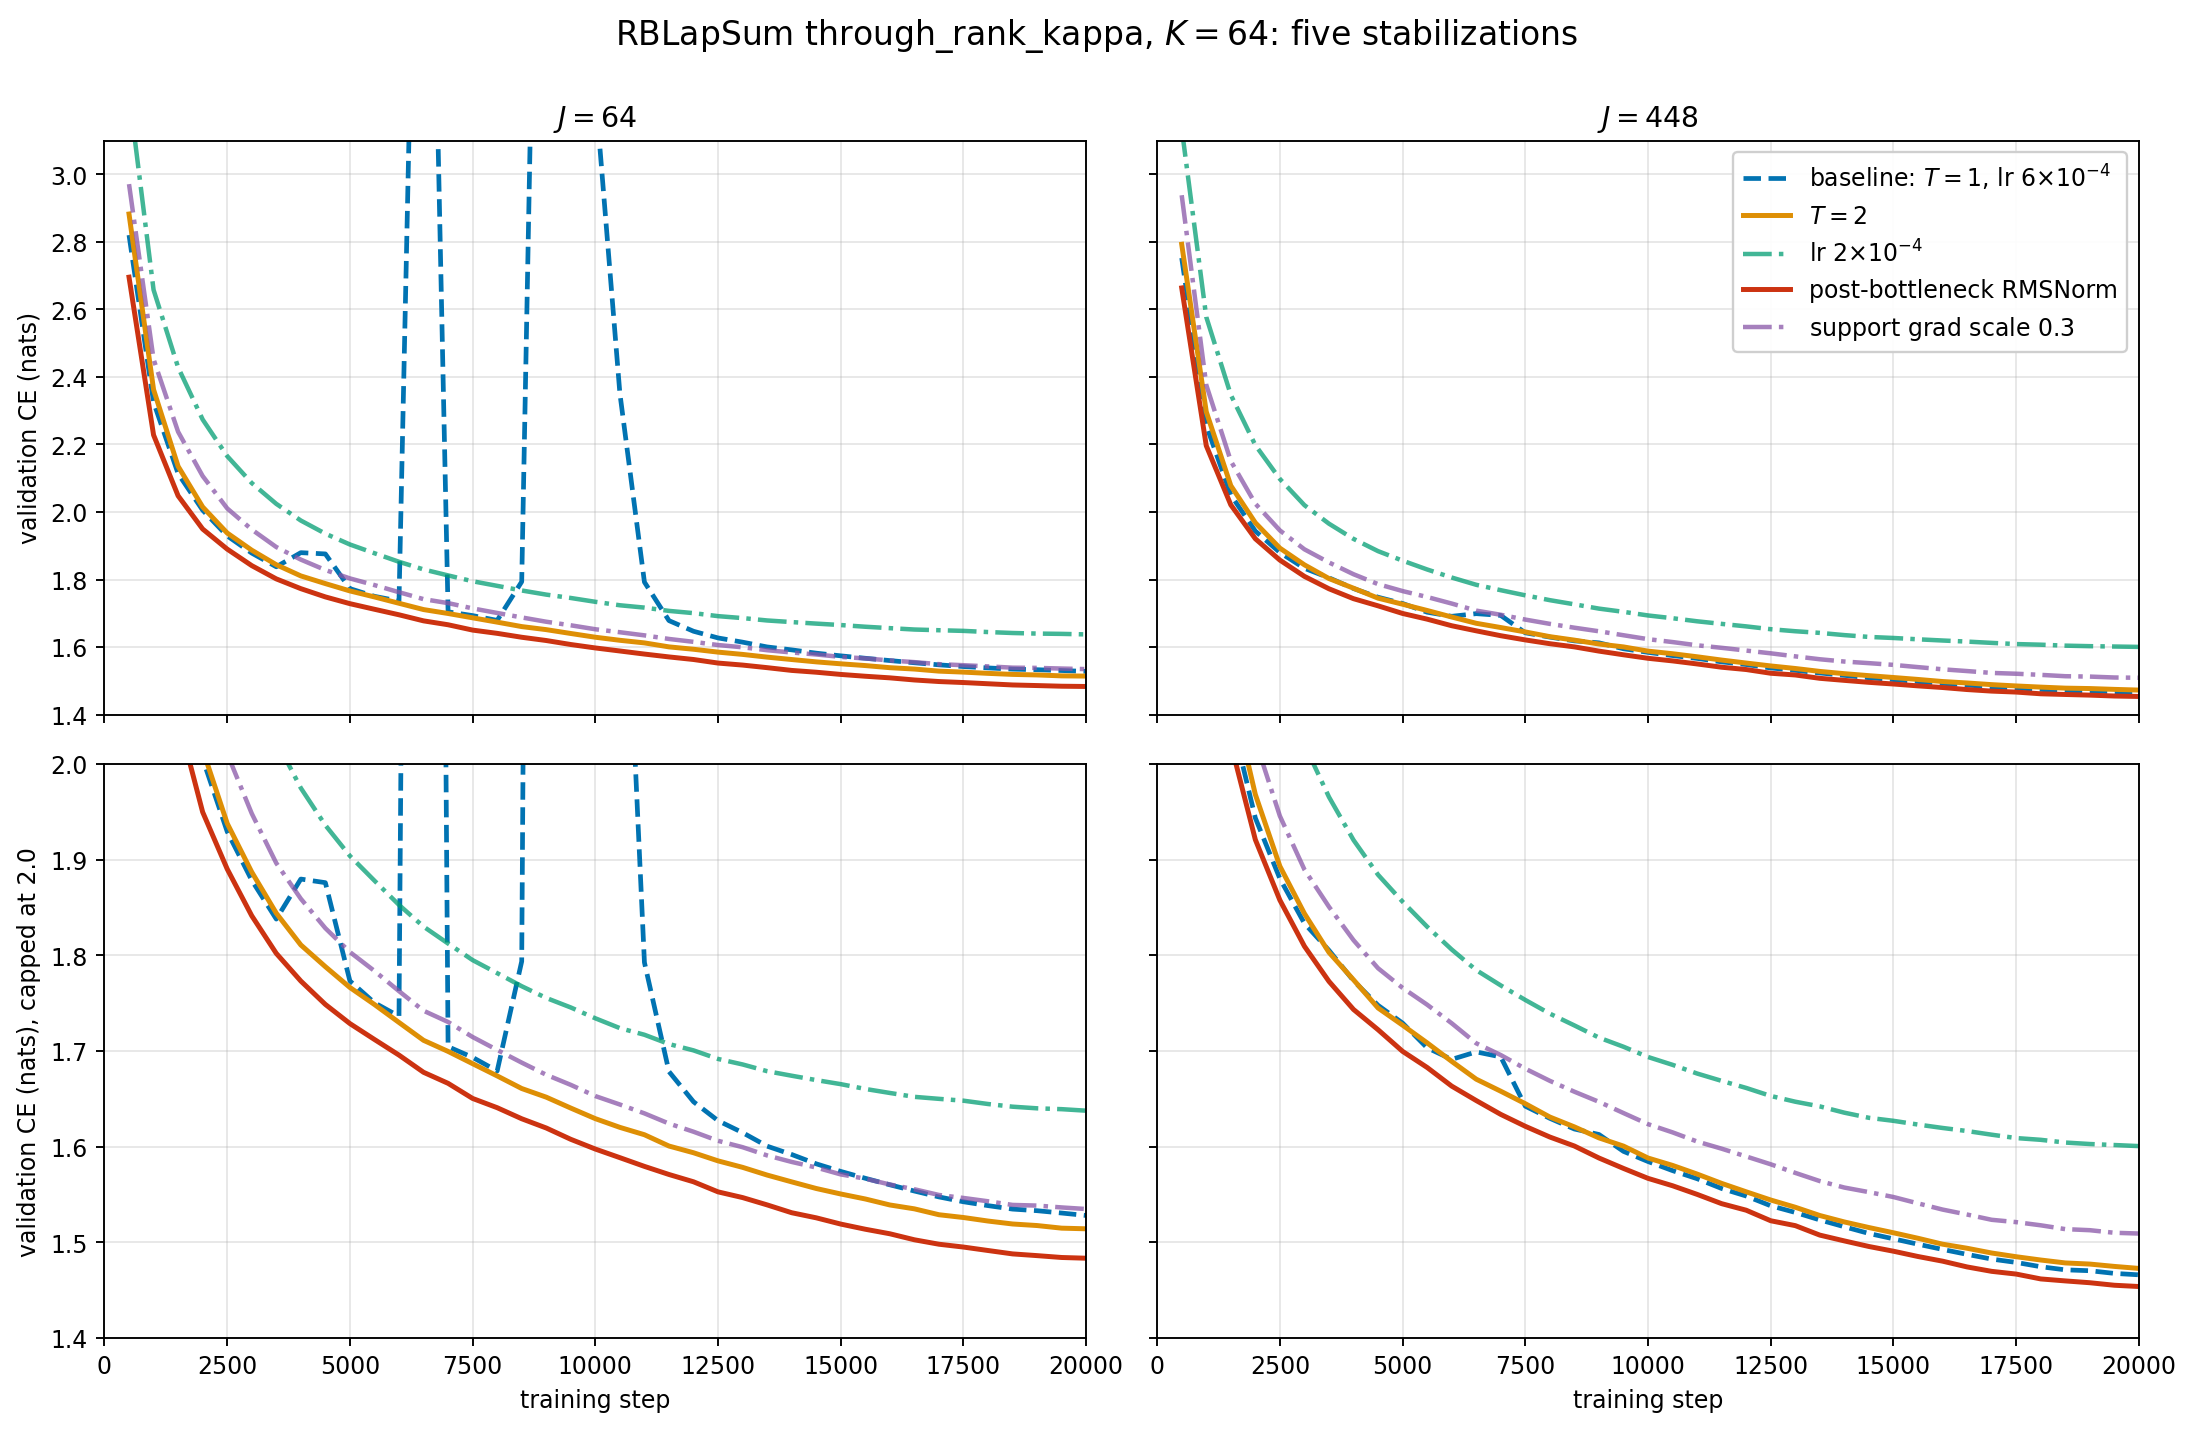
\includegraphics[width=\textwidth]{figures/stab_k64.png}
\caption{$K=64$, panels as above. No run diverges, but the baseline
(blue, $J=64$) leaves the plotted range twice and returns -- the recovered
excursion discussed in the text. The output RMSNorm is best at both $J$,
by $0.012$--$0.045$ nats over the baseline; the capped row makes the
ordering of the four arms legible over the second half of training.}
\end{figure}

\begin{figure}[h]\centering
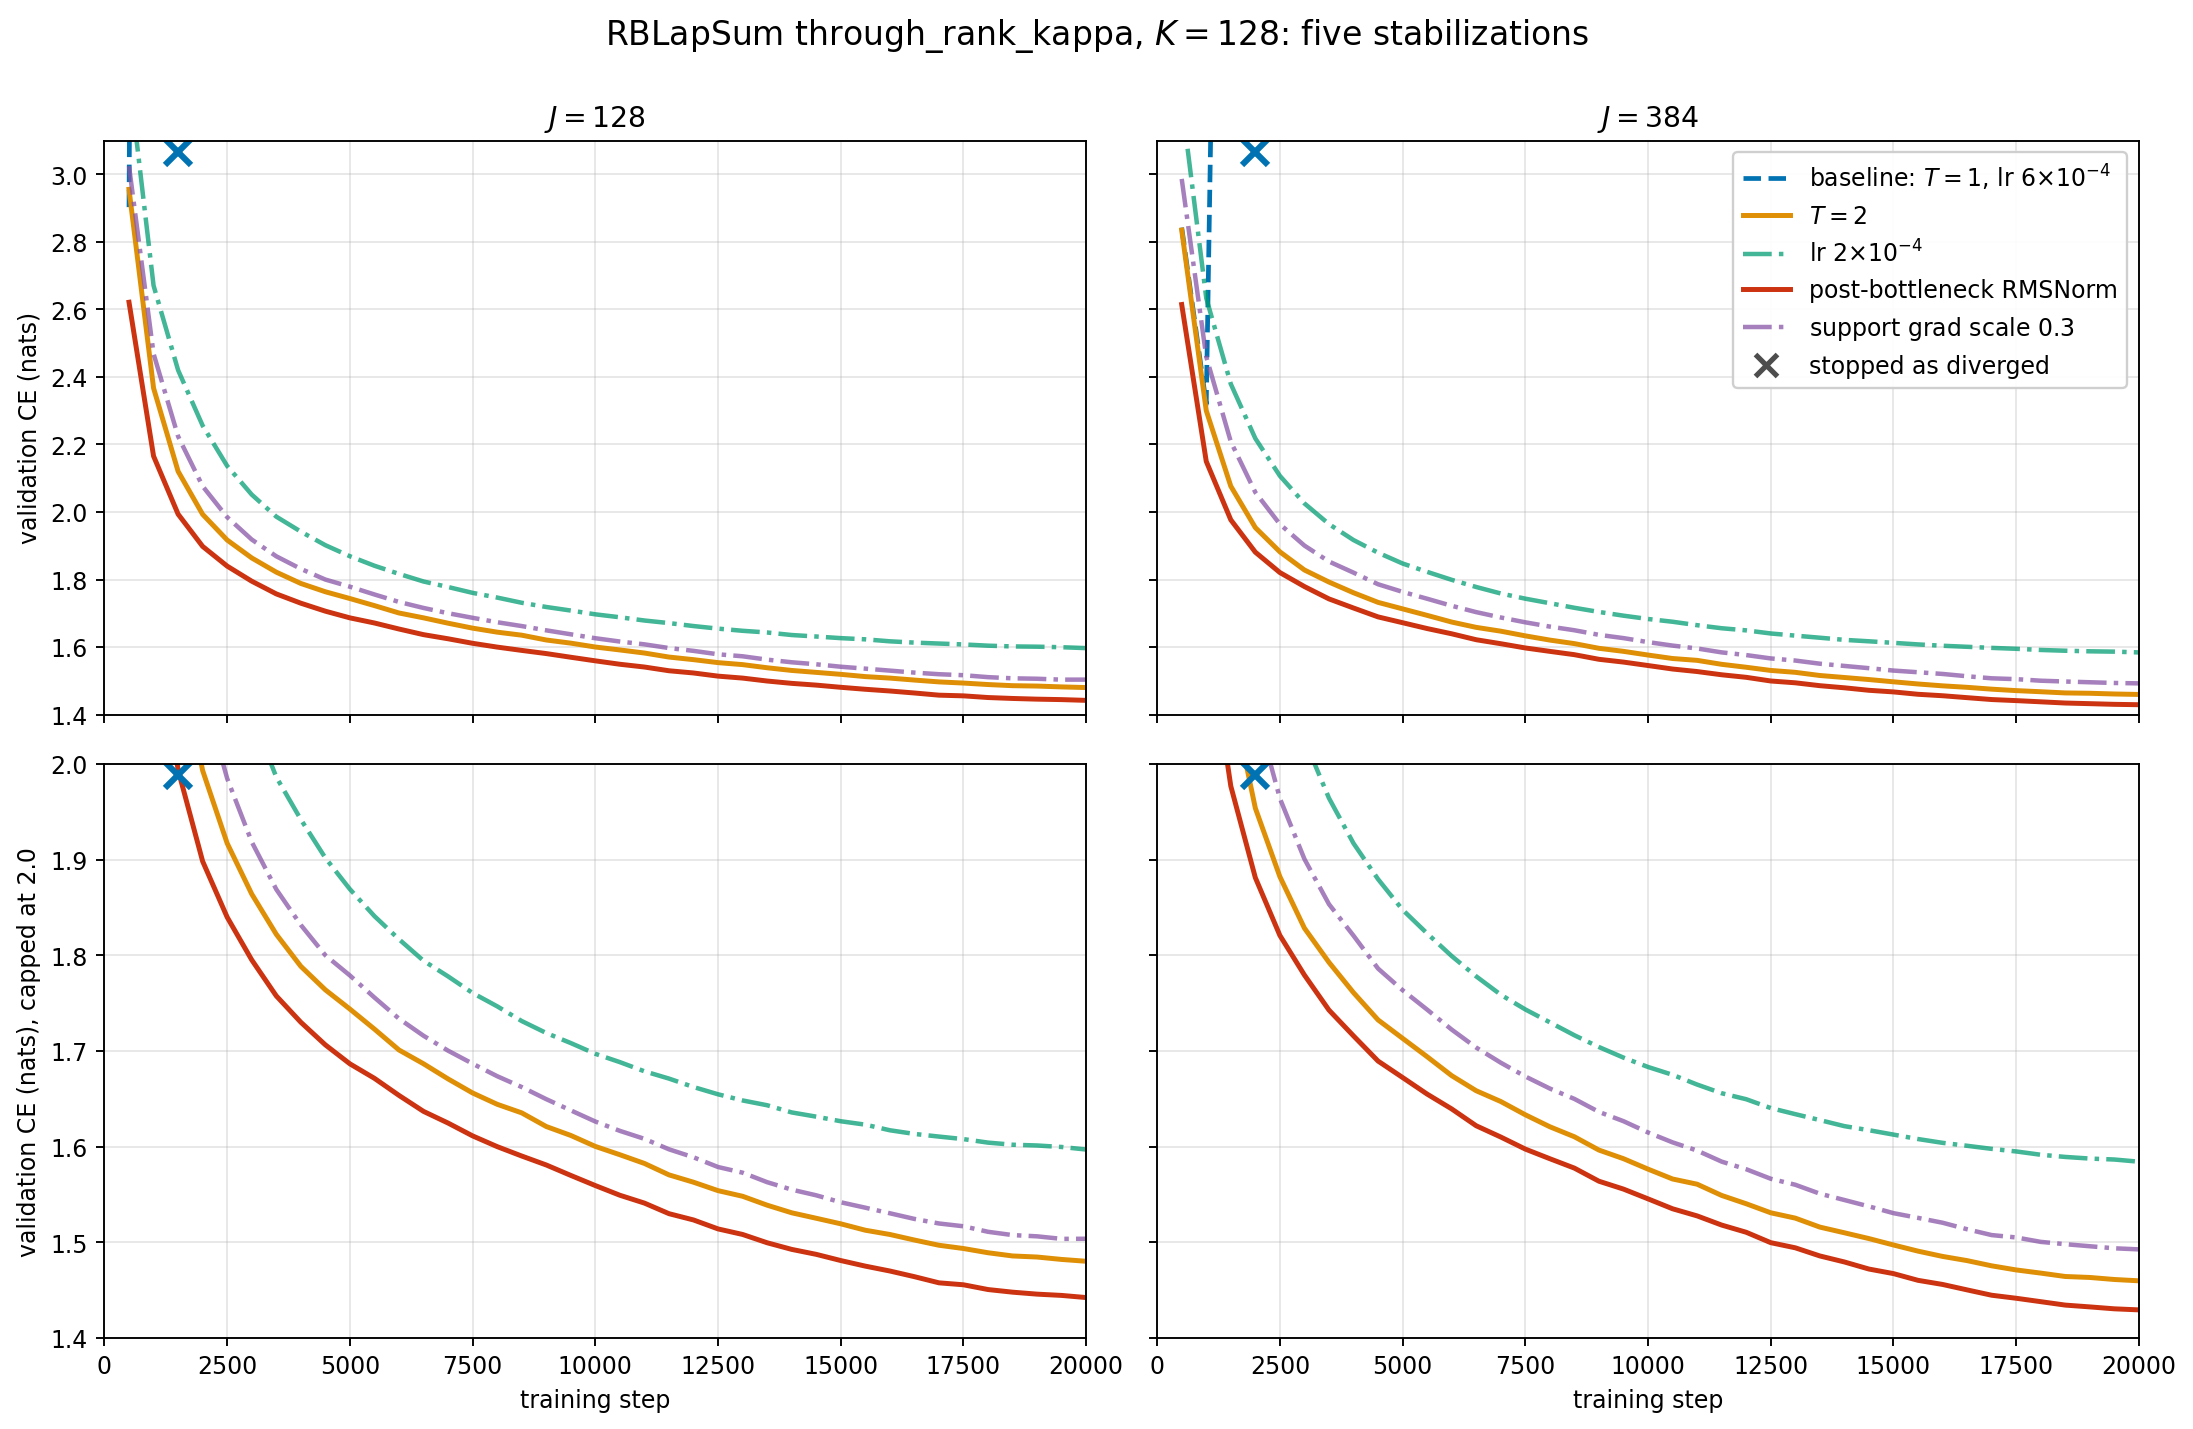
\includegraphics[width=\textwidth]{figures/stab_k128.png}
\caption{$K=128$, panels as above. The baseline (blue) diverges at both
$J$ and leaves the plotted range, its stop marked by a cross at the top
edge of each panel. All four interventions converge, and the ordering is
the same at both $J$ and stable from about step 3000: the output RMSNorm
(red) runs lowest throughout, ahead of $T=2$, then the support-gradient
scale, then the reduced learning rate.}
\end{figure}

\paragraph{A recovered excursion.}
The baseline at $(64,64)$ survives but is visibly marginal. Its validation
CE rises from $1.74$ to $5.12$ at step 6500 and recovers within 500 steps,
rises again to $5.60$ at step 9000, and decays back below $1.8$ by step
11000, ending at its own best value, $1.5281$. No other surviving run
behaves this way: the only other runs above CE $2.0$ after step 3000 are
the two slowest reduced-learning-rate runs, which are simply behind rather
than excursing. This is the burst-and-recover behaviour the divergence
guard's 800-step window is meant to tolerate, and it places the baseline at
the edge of stability one configuration earlier than the divergences alone
would suggest.

\paragraph{Where the arms differ.}
Relative to the output RMSNorm, aggregated over the configurations in which
both runs converged:

\begin{center}\small
\begin{tabular}{lcc}
\toprule
arm & gap to post-norm (nats) & configurations \\
\midrule
baseline            & $-0.047$ to $+0.045$ & 4 (diverges in 2) \\
$T=2$               & $-0.043$ to $+0.038$ & 6 \\
support grad $0.3$  & $+0.005$ to $+0.063$ & 6 \\
lr $2\times10^{-4}$ & $+0.080$ to $+0.155$ & 6 \\
\bottomrule
\end{tabular}
\end{center}

The baseline and $T=2$ straddle zero: they beat the RMSNorm at
$(32,480)$ by $0.047$ and $0.043$ nats respectively and lose to it
everywhere else. The other two arms are behind in every configuration.

\paragraph{The hard bottleneck.}
Two hard-AbsTopK runs with the same output RMSNorm test whether the norm
helps where there is no surrogate gradient and no instability. Against the
matched runs from the earlier campaign (same configuration and seed, no
norm):

\begin{center}\small
\begin{tabular}{lccc}
\toprule
$K$ & without post-norm & with post-norm & difference \\
\midrule
$32$  & 1.6162 & 1.6022 & $-0.0140$ \\
$512$ & 1.4298 & 1.4232 & $-0.0066$ \\
\bottomrule
\end{tabular}
\end{center}

Both improve. The norm is therefore not compensating for the surrogate;
it improves a bottleneck that has no surrogate at all.

% ============================================================
\section{Interpretation}
% ============================================================

The ordering is consistent with the initialization measurement in
\code{docs/init-pi-grid.pdf} and \code{docs/init-pi-grid-postnorm.pdf}.
Under \code{residual\_out} each block replaces the residual stream, so the
bottleneck's output scale compounds through depth: at $K=512$ the pre-gate
score RMS runs $1.67\to6.16\to13.3$ across blocks 0, 4 and 7 at
initialization, and the surrogate gain $\Pi$ with it,
$262\to1089\to2384$. Adding the output RMSNorm holds the score RMS at
$1.67\to1.79\to1.82$ and $\Pi$ at $262\to288\to293$: the deep-block gain
falls by a factor of eight and becomes depth-uniform.

That is a different kind of fix from the other three. Broadening the
kernel, shrinking the step and damping the support term all reduce the
\emph{size of the surrogate contribution}; the norm removes the
\emph{amplification} that made the contribution dangerous in deep blocks,
leaving the gradient itself intact. The measured costs follow: the three
attenuating arms pay between $0.03$ and $0.16$ nats, while the norm pays
nothing and usually gains.

The support-gradient-scale result is worth stating explicitly, because it is the
intervention the earlier counterfactual experiments identified as causally
effective: disabling the support gradient stopped both burst initiation and
post-collapse inflation. It does stabilize here -- six configurations, no
divergences -- but at $0.3$ it costs $0.005$--$0.063$ nats relative to the
norm and is worse than the untouched baseline wherever the baseline
survives. Attenuating the boundary exchange removes the instability and
part of the learning signal together.

% ============================================================
\section{Recommendation and scope}
% ============================================================

For the configurations tested, the output RMSNorm is the intervention to
prefer: it is the only one that stabilizes the $K=128$ rows without paying
for it, it is best in five of six configurations, and it also improves the
hard bottleneck. Where an architectural change is unwanted, $T=2$ is the
next best option and costs little.

Scope. All cells are single runs at one seed, and earlier work in this
project showed that divergence at marginal configurations is stochastic, so
individual outcomes should be read as draws from a divergence rate rather
than as deterministic verdicts; the patterns that repeat across
configurations -- the baseline being the only arm that diverges, the
RMSNorm leading in five of six, the reduced learning rate being uniformly
last -- are the robust part. Only one support-gradient-scale value ($0.3$) and one
reduced learning rate ($2\times10^{-4}$) were tested, so neither arm is
tuned; a milder support-gradient scale in particular might retain the stabilization
at a smaller accuracy cost. Finally, the single configuration in which the
untouched baseline is best, $(32,480)$, is also the least stressed one, so
the norm should be read as a fix for stressed configurations rather than a
universal improvement.

\end{document}
